%%%%%%%%%%%%%%%%%%%%%%%%%%%%%%%%%%%%%%%%%
% Short Sectioned Assignment
% LaTeX Template
% Version 1.0 (5/5/12)
%
% This template has been downloaded from:
% http://www.LaTeXTemplates.com
%
% Original author:
% Frits Wenneker (http://www.howtotex.com)
%
% License:
% CC BY-NC-SA 3.0 (http://creativecommons.org/licenses/by-nc-sa/3.0/)
%
%%%%%%%%%%%%%%%%%%%%%%%%%%%%%%%%%%%%%%%%%

%----------------------------------------------------------------------------------------
%	PACKAGES AND OTHER DOCUMENT CONFIGURATIONS
%----------------------------------------------------------------------------------------

\documentclass[paper=a4, fontsize=11pt]{scrartcl} % A4 paper and 11pt font size

\usepackage[T1]{fontenc} % Use 8-bit encoding that has 256 glyphs
\usepackage{fourier} % Use the Adobe Utopia font for the document - comment this line to return to the LaTeX default
\usepackage[english]{babel} % English language/hyphenation
\usepackage{amsmath,amsfonts,amsthm} % Math packages
\usepackage{lipsum}
\usepackage{graphicx}

\usepackage{sectsty} % Allows customizing section commands
\allsectionsfont{\centering \normalfont\scshape} % Make all sections centered, the default font and small caps

\usepackage{fancyhdr} % Custom headers and footers
\pagestyle{fancyplain} % Makes all pages in the document conform to the custom headers and footers
\fancyhead{} % No page header - if you want one, create it in the same way as the footers below
\fancyfoot[L]{} % Empty left footer
\fancyfoot[C]{} % Empty center footer
\fancyfoot[R]{\thepage} % Page numbering for right footer
\renewcommand{\headrulewidth}{0pt} % Remove header underlines
\renewcommand{\footrulewidth}{0pt} % Remove footer underlines
\setlength{\headheight}{13.6pt} % Customize the height of the header

\numberwithin{equation}{section} % Number equations within sections (i.e. 1.1, 1.2, 2.1, 2.2 instead of 1, 2, 3, 4)
\numberwithin{figure}{section} % Number figures within sections (i.e. 1.1, 1.2, 2.1, 2.2 instead of 1, 2, 3, 4)
\numberwithin{table}{section} % Number tables within sections (i.e. 1.1, 1.2, 2.1, 2.2 instead of 1, 2, 3, 4)

\setlength\parindent{0pt} % Removes all indentation from paragraphs - comment this line for an assignment with lots of text

%----------------------------------------------------------------------------------------
%	TITLE SECTION
%----------------------------------------------------------------------------------------

\newcommand{\horrule}[1]{\rule{\linewidth}{#1}} % Create horizontal rule command with 1 argument of height

\title{	
\normalfont \normalsize 
\textsc{Columbia University -- Computer Vision Spring 13'} \\ [25pt] % Your university, school and/or department name(s)
\horrule{0.5pt} \\[0.4cm] % Thin top horizontal rule
\huge Homework One \\ % The assignment title
\horrule{2pt} \\[0.5cm] % Thick bottom horizontal rule
}

\author{Joseph Ellis} % Your name

\date{\normalsize\today} % Today's date or a custom date

\begin{document}

\maketitle % Print the title

%----------------------------------------------------------------------------------------
%	PROBLEM 1
%----------------------------------------------------------------------------------------

\section{Problem Number One}

\subsection{Part 1}
This graph represents the focus difference as a function of the object distance from the focal length of the lens.
For Figure \ref{Part 1}, the following values were used in creation of the figure: \begin{math} f = 100,\end{math} and \begin{math}z_{i}\end{math} ranges from \begin{math} 105-150\end{math}.
The actual units of the values are the same throughout and are not important to the calculations.

%Add the figure
\begin{figure}
\centering
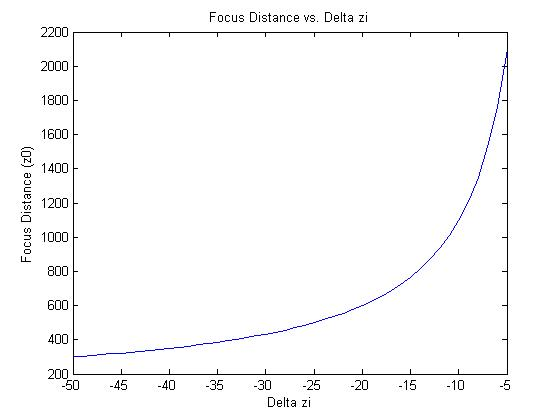
\includegraphics[width=3in]{prob11.jpg}
\caption{Focus Distance vs. \begin{math}z_{i}-f\end{math}}
\label{Part 1}
\end{figure}

\subsection{Part 2}
For this problem we calculated the depth of the field as a function of image distance from the lens.
The values used to create Figure \ref{Part 2} are as follows: \begin{math}z_{0} = 100, f = 50, d = 100,\end{math} and the graph below depicts the blur when the image is between \begin{math}80\end{math} and \begin{math}120\end{math}.
The allowable confusion circle depicted on the graph is equal to \begin{math}15\end{math}.
The actual units of the values are the same throughout and are not important to the calculations.

%Add the figure
\begin{figure}
\centering
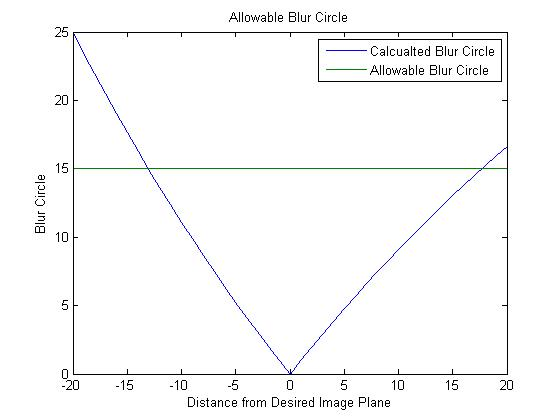
\includegraphics[width=3in]{prob12.jpg}
\caption{Confusion Circle Radius vs. \begin{math}z_{0prime}-z_{0}\end{math}}
\label{Part 2}
\end{figure} 

\subsection{Part 3}

In this problem we attempted to recreate the depth of field lines seen on a camera with variable focus.
These lines demonstrate the distance that images can be for a given focus distance and object distance available
In Figure \ref{Part 3} the diameter of the lens was set to \begin{math}4\end{math} and the allowable blur circle was \begin{math}.02\end{math}.
The focus distances plotted can be seen in the figure, as well as the object distances for which we found the depth of field.

\begin{figure}
\centering
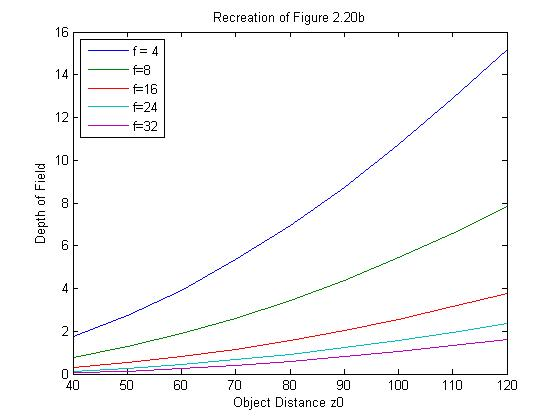
\includegraphics[width=3in]{prob13.jpg}
\caption{Depth of Field vs. Object Distances for a Variety of Focal lengths}
\label{Part 3}
\end{figure} 


\section{Problem Number Two}

The derivation of the equation \begin{math}f^{2}=(i-f)(o-f)\end{math} can be seen below.

\begin{align} 
\begin{split}
f = \frac{io}{i+o}\\	
i-f = \frac{i}{1}+\frac{io}{i+o} = \frac{(i(i+o)-io)}{i+o} = \frac{i^{2}}{i+o}\\	
o-f =\frac{o}{1}+\frac{io}{i+o} = \frac{(o(i+o)-io)}{i+o} = \frac{o^2}{i+o}\\.
f^{2}=(\frac{io}{i+o})^{2}\\
&=\frac{i^{2}o^{2}}{(i+o)^{2}}\\
&=\frac{(i(i+o) -io)(o(i+o)-io)}{(i+o)^2}\\
&= \frac{(i(i+o)-io)}{i+o}* \frac{(o(i+o)-io)}{i+o}\\
&=(i-f)(o-f)
\end{split}					
\end{align}

%------------------------------------------------

\subsection{Problem Number Three}

Please see Matlab Script outputs generated from CVAssignment1.m.

%------------------------------------------------

\subsection{Problem Number Four}

This problem was worked out by hand and presented to the Teaching Assistants.

%------------------------------------------------

\subsection{Problem Number Five}

This problem was worked out by hand and presented to the Teaching Assistants.


%----------------------------------------------------------------------------------------

\end{document}